\section{Wavelet-based generative framework}

\subsection{Wavelet representation of RTI fields}

The wavelet pipeline begins with the preprocessing of the RTI dataset. The raw
density fields are first loaded from the simulation files and preprocessed
using the existing data augmentation routines. A two-dimensional discrete
wavelet transform is then applied to each image using a Daubechies-1 basis.

For a decomposition level $j$, each field is mapped to four coefficient maps:
the approximation coefficients $c_A$ and the horizontal, vertical, and
diagonal detail coefficients $c_H$, $c_V$, and $c_D$. In the implementation,
these four arrays are stacked into a tensor of shape $(N,4,H',W')$, where $N$
is the number of samples and $(H',W')$ is the spatial size of the wavelet
coefficients at the chosen level. The dataset is then split into training,
validation, and test subsets, and each split is saved independently as a PyTorch
tensor.

This representation preserves the most relevant multi-scale information while
reducing the learning problem to a structured tensor prediction task. In
practice, the decomposition also makes the notion of coarse-to-fine generation
explicit: the approximation channel plays the role of a low-frequency prior,
while the three detail channels contain the higher-frequency content that must
be synthesized.

\subsection{Conditional diffusion on wavelet coefficients}

The training data are loaded from the precomputed tensors and normalized
channel by channel using the statistics of the training split. This
normalization is important because the four wavelet channels do not share the
same numerical scale and would otherwise contribute unevenly to the
optimization process.

The model uses a conditional DDPM structure. The input to the U-Net is composed
of the approximation channel concatenated with the noisy detail channels. The
network predicts the noise applied to the detail coefficients, which means that
generation is guided by the coarse-scale information rather than being
unconditional. In other words, the model learns how to reconstruct the missing
fine-scale structure given the large-scale wavelet content.

The corresponding architecture is deliberately compact. The U-Net receives
four input channels in total, with one channel reserved for the prior
information and three channels corresponding to the target detail maps. The
network depth and the number of blocks per level remain modest so that training
is compatible with the size of the available RTI dataset. The diffusion
schedule itself follows the same principle as the baseline model, with a
discretized Markov process controlled by a linear noise schedule between
\texttt{min\_beta} and \texttt{max\_beta}.

During training, the loss is again the standard mean squared error between the
true noise and the noise predicted by the network. The model therefore learns a
denoising function conditioned on the coarse wavelet coefficients. Once
training is complete, the checkpoint and the preprocessing statistics are
stored in a configuration file so that sampling can be reproduced later without
ambiguity.

\begin{figure}[H]
    \centering
    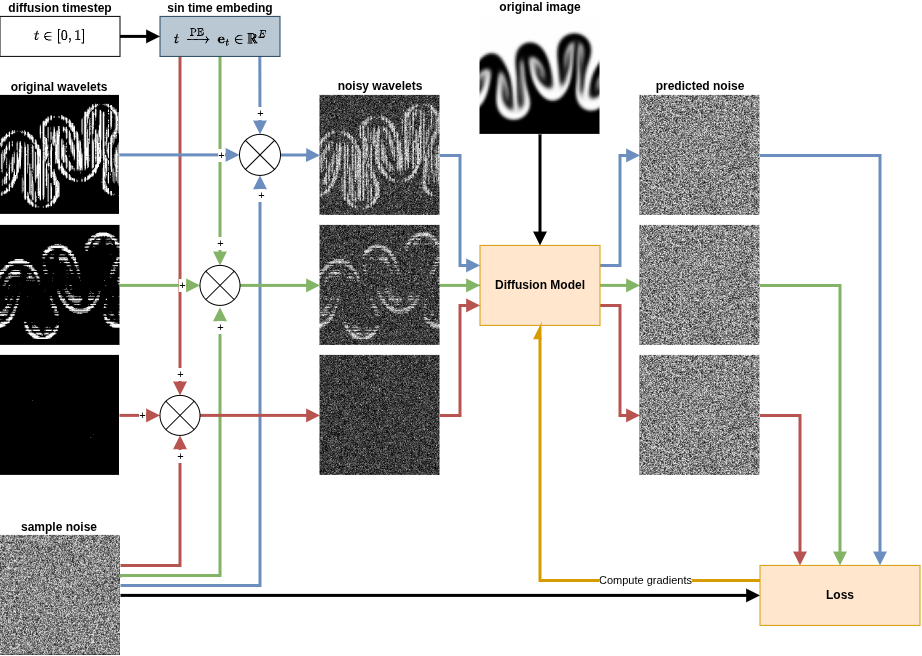
\includegraphics[width=0.88\textwidth]{figures/ch4/training_loop_conditioned.drawio.png}
    \caption{Training loop for the conditional wavelet DDPM. The approximation coefficients are kept as conditioning information, while noise is added only to the detail channels that the network must denoise.}
    \label{fig:conditioned_training_loop}
\end{figure}

% \subsection{Generation procedure}

% The generation stage loads the trained checkpoint and the associated
% normalization parameters. A batch of wavelet coefficients is sampled from the
% validation set and the approximation channel is extracted as a condition.
% Starting from the conditional prior, the DDPM iteratively denoises the target
% detail channels and produces a synthetic coefficient tensor.

% The generated coefficients are then denormalized and saved to disk. This file
% can subsequently be converted back to image space by inverting the wavelet
% transform, which makes it possible to compare the generated fields with the
% reference RTI simulations both visually and quantitatively.

% Because the generation is conditioned on the low-frequency part of an existing
% sample, the model is not asked to invent the global structure from scratch. It
% instead focuses on reconstructing plausible local details compatible with the
% coarse-scale organization of the flow. This is a natural strategy for RTI
% fields, where the large-scale morphology strongly constrains the admissible
% small-scale fluctuations.

